%====================================================================================
\section{Definición}
%====================================================================================

%------------------------------------------------------------------------------------
\subsection{Origen de la endogeneidad}
%------------------------------------------------------------------------------------

\begin{frame}{Situaciones que originan endogeneidad}
	\begin{enumerate}
		\item Variables omitidas
			\begin{itemize}
				\item Modelo verdadero: $y_i=x_{i1}'\beta_1+x_{i2}'\beta_2+\nu_i$
				\item Modelo estimado: $y_i=x_{i1}'\beta_1+\mu_i$
			\end{itemize}
		\item Doble causalidad o simultaneidad
			\begin{align*}
				y_i &= z_{i}\beta_1+x_{i}\beta_2+\nu_{i} \\
				x_i &= z_{i}\gamma_1+y_{i}\gamma_2+\mu_{i}
			\end{align*}
		\item Errores de medida
				\begin{itemize}
					\item Modelo verdadero: $y_i=x_{i}^*\beta+\nu_i$
				\end{itemize}
			  Pero existe un error de medida tal que el valor observado de $x$ es: $x_i = x_i^*+\epsilon$
				\begin{itemize}
					\item Modelo estimado: $y_i=x_{i}\beta+\mu_i$
				\end{itemize}
	\end{enumerate}
\end{frame}

%------------------------------------------------------------------------------------
\subsection{Variable instrumental}
%------------------------------------------------------------------------------------

\begin{frame}{Variable instrumental}
	\begin{figure}[H]
		\begin{centering}
			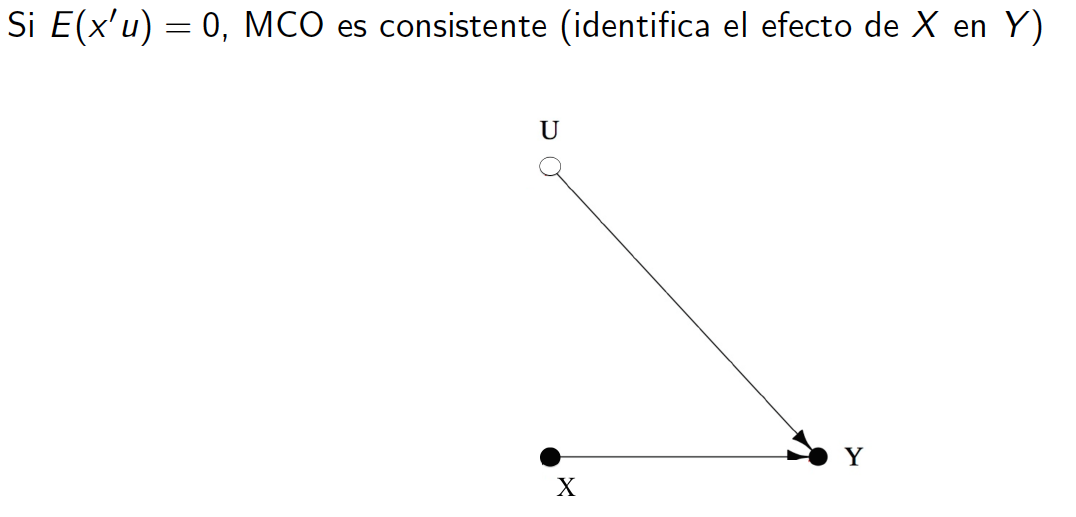
\includegraphics[scale=0.25]{fig/fig1.png}
		\end{centering}
	\end{figure}
\end{frame}
%---------------------------------------------------
\begin{frame}{Variable instrumental}
	\begin{figure}[H]
		\begin{centering}
			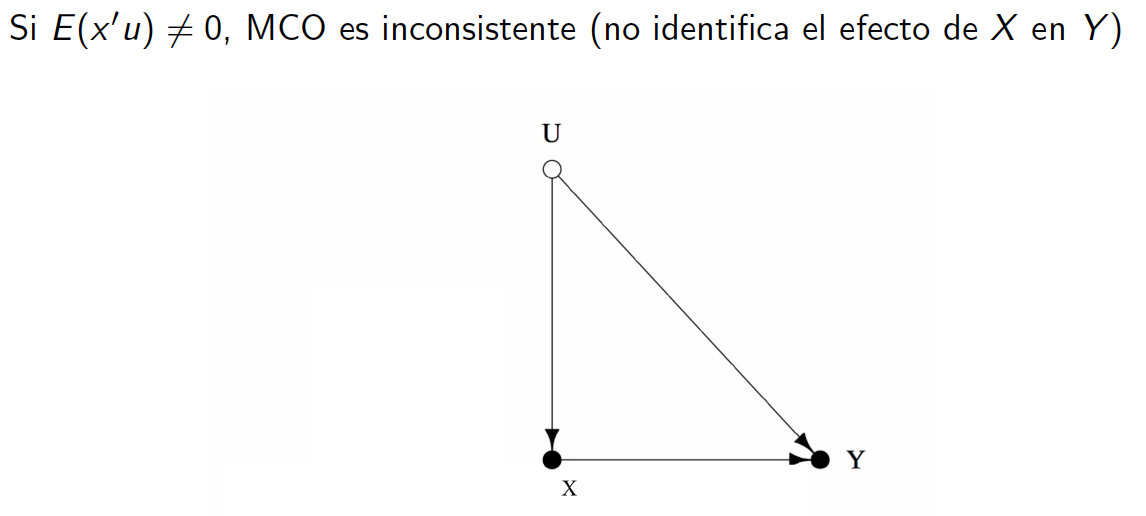
\includegraphics[scale=0.25]{fig/fig2.png}
		\end{centering}
	\end{figure}
\end{frame}
%---------------------------------------------------
\begin{frame}{Variable instrumental}
	\begin{figure}[H]
		\begin{centering}
			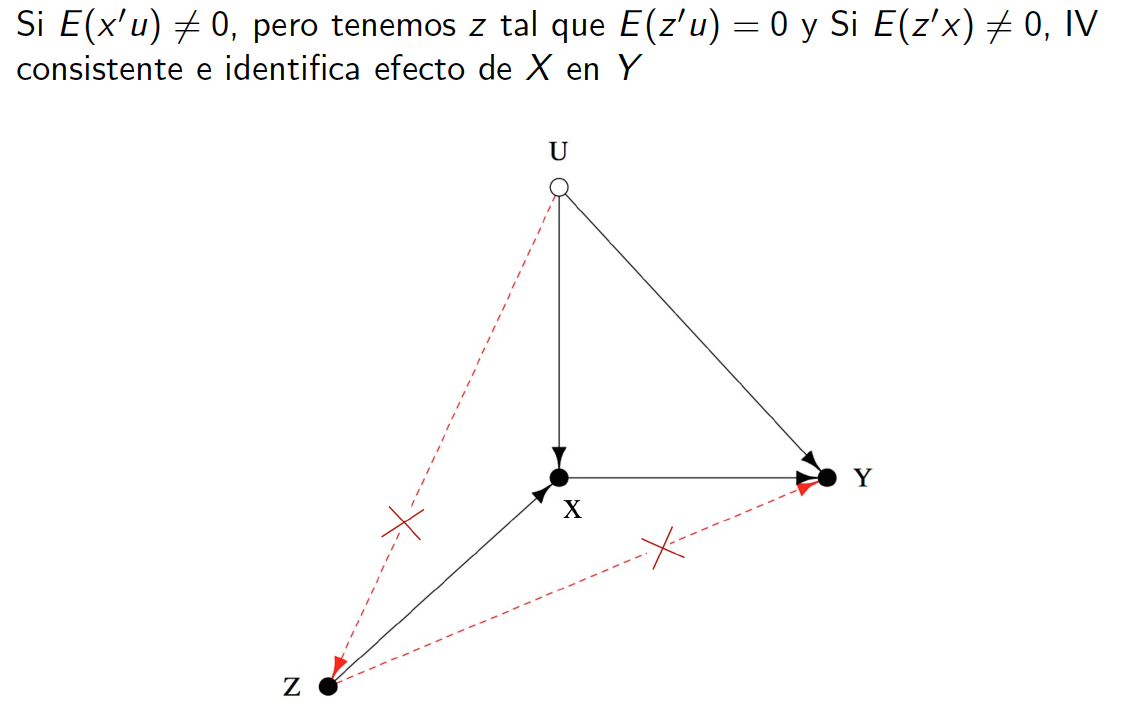
\includegraphics[scale=0.25]{fig/fig3.png}
		\end{centering}
	\end{figure}
\end{frame}
%---------------------------------------------------
\begin{frame}{Variable instrumental}
	\begin{itemize}
		\item Un instrumento es una de las formas de resolver el problema de endogeneidad.
		\item Dado el modelo $y_i=\beta_0+\beta_1 x_i+\mu_i$. Existe una variable $z$ que cumple con el siguiente diagrama:
			\begin{description}
				\item[Condición de Relevancia:] $Cov(zx) \neq 0$
				\item[Condición de Exogeneidad:] $Cov(z\mu) = 0$
			\end{description}
	\end{itemize}
\end{frame}

%------------------------------------------------------------------------------------
\subsection{Ejemplo}
%------------------------------------------------------------------------------------
\begin{frame}{Educación y salud\footnote{Adaptado de Lee (2005), \emph{Micro-Econometrics for Policy, Program, and Treatment Effects}. Pág. 129.}}
	\begin{itemize}
		\item Imagine un programama de salud que ofrece educación ($z$) sobre los beneficios de los ejercicios.
		\item Imagine que estamos interesados en los efectos del ejercicio ($d$) sobre la la salud ($y$), y no de los efectos de $z$ sobre $y$.
		\item Se tiene entonces una situación donde:
			\begin{equation*} 
				z \rightarrow d \rightarrow y
			\end{equation*}
		\item La educación por si misma es improbable que afecte directamente a la salud.
		\item La variable $z$ que afecta a $d$ pero no a $y$ directamente es llamada un 
		\emph{instrumento}.
	\end{itemize}
\end{frame}